\documentclass[11pt,a4paper]{article}
\usepackage[margin=2.5cm]{geometry}
\usepackage{amsmath,amssymb,booktabs,graphicx,xcolor,hyperref,microtype}
\usepackage{authblk}
\hypersetup{colorlinks=true,linkcolor=blue,citecolor=blue,urlcolor=blue}

\newcommand{\Corder}{C_{\mathrm{order}}}
\newcommand{\sw}{\sigma_w}
\newcommand{\na}{\mathrm{na\_ratio}}
\newcommand{\Pcausal}{P_{\mathrm{causal}}}
\newcommand{\Psp}{P_{\mathrm{spatial}}}
\newcommand{\Ptemp}{P_{\mathrm{temporal}}}

\title{\textbf{Paper 58: Empirical Causal Purity and the Two-Dimensional Identity Condition}\\
\large Spatial and Temporal Causal Purity as\\
Jointly Necessary Conditions for Stable Identity}

\author[1]{Gabriel Aubin-Moreau}
\affil[1]{Independent research}
\date{March 2026}

\begin{document}
\maketitle

\begin{abstract}
Paper~57 introduced causal purity $\Pcausal$ --- the fraction of a cell's
pre-consolidation wave-contact events originating from the same zone --- as
the substrate-agnostic primitive underlying the noise-floor condition.
Its key claim: $\dot{\Corder}>0$ iff $\Pcausal > p_c$.

We implement direct empirical measurement of $\Pcausal$ in the VCML simulation:
for every fieldM consolidation event, we record whether the triggering wave's zone
matches the consolidating cell's zone.
No geometric approximation. No spatial distance.

\textbf{Finding 1 (expected):}
Empirical $\Pcausal$ matches the geometric prediction and varies with $r_\mathrm{wave}$
as expected: 0.88--0.98 across conditions, lower at large $r_\mathrm{wave}$.

\textbf{Finding 2 (surprising):}
C\_perturb and C\_ref have \emph{nearly identical} spatial $\Pcausal$ at the same
$r_\mathrm{wave}$ (within 0.02--0.03).
Yet C\_ref $\sigma_w$ is 3--10$\times$ higher than C\_perturb $\sigma_w$.
Spatial causal purity alone does not explain the write-policy difference.

\textbf{Finding 3:}
For C\_perturb only, $\sigma_w \approx A(1-\Pcausal)$ (ratio constant across
all $r_\mathrm{wave}$, $A \approx 0.84$).
For C\_ref, $\sigma_w \gg A(1-\Pcausal)$: additional noise not accounted for
by spatial zone matching.

\textbf{Conclusion:}
The causal purity framework requires a second dimension.
Write policy determines \emph{temporal} causal purity $\Ptemp$: whether the
consolidation event happens \emph{during} active wave contact from the same zone,
vs.\ \emph{after} the wave has passed.
C\_perturb sets $\Ptemp=1$ by construction (writes only during $w_a>0.05$).
C\_ref has $\Ptemp \ll 1$ (writes during quiescence, after causal events have faded).

The substrate-agnostic identity condition is:
\begin{equation*}
  \dot{\Corder} > 0
  \iff
  \Psp > p_c^\mathrm{sp} \;\text{ AND }\; \Ptemp > p_c^\mathrm{temp},
\end{equation*}
with no spatial geometry in the final statement.
\end{abstract}

%──────────────────────────────────────────────────────────────────────────────
\section{Introduction}

Paper~57 derived a geometric approximation for $\Pcausal$ and showed that
$\sigma_w \approx (2/\delta) V_\mathrm{bnd}$ under C\_perturb.
It then proposed that the true primitive is the causal graph of influence
rather than wave geometry.

The logical next step is direct empirical measurement: instrument the simulation
to record, at each consolidation event, which zone triggered the write.
Paper~57 predicted $\sigma_w \propto (1-\Pcausal)$ for C\_perturb.
The question: does the same equation hold for C\_ref at equal $\Pcausal$?
If yes, spatial causal purity is the sufficient predictor.
If no, there is an additional dimension.

We run C\_perturb and C\_ref at $r_\mathrm{wave} \in \{2,4,8,10\}$, S2 sub-threshold,
measuring $\Pcausal$ empirically at each consolidation event.

%──────────────────────────────────────────────────────────────────────────────
\section{Method: Empirical Causal Purity Measurement}

\paragraph{Spatial causal purity $\Psp$.}
For each consolidation event at cell $i$:
\begin{itemize}
  \item Under C\_perturb: cell $i$ writes when $\mathrm{streak}_i \geq \mathrm{SS}$
    and $w_a[i] > 0.05$. The active wave class $\mathrm{wc}[i]$ is the exact causal zone.
  \item Under C\_ref: cell $i$ writes when $\mathrm{streak}_i \geq \mathrm{SS}$.
    The last observed wave class $\mathrm{wc\_last}[i]$ is used as a proxy for the
    causal zone (updated whenever $w_a[i] > 0.05$).
\end{itemize}
In both cases,
\begin{equation}
  \Psp = \frac{\text{number of writes where } z_\mathrm{wave} = z_\mathrm{cell}}
             {\text{total writes}},
\end{equation}
accumulated over all 3000 steps (no geometric approximation).

\paragraph{Temporal causal purity $\Ptemp$.}
Implicitly, C\_perturb has $\Ptemp = 1$: every write occurs during the causal
wave event.
C\_ref has $\Ptemp < 1$: writes occur at the start of each calm period, after
the causal wave has moved on.
$\Ptemp$ is \emph{not} derived from tracking which wave caused which write ---
rather, it is the categorical difference in write-trigger logic between the two modes.

%──────────────────────────────────────────────────────────────────────────────
\section{Results}

\begin{table}[h]
\centering
\caption{Empirical $\Psp$, $\sigma_w$, and identity outcome at step~3000.
For each condition: mean over 5 seeds. $\delta = W_\mathrm{zone}/r_\mathrm{wave} = 20/r$.}
\label{tab:main}
\begin{tabular}{llrrrrrr}
\toprule
Mode & $r$ & $\delta$ & $\Psp$ & $1-\Psp$ & $\sigma_w$ & $\sigma_w/(1-\Psp)$ & na \\
\midrule
CP  & 2  & 10.0 & 0.981 & 0.019 & 0.0111 & 0.577 & 1.261 \\
CP  & 4  &  5.0 & 0.948 & 0.052 & 0.0452 & 0.861 & 1.140 \\
CP  & 8  &  2.5 & 0.905 & 0.095 & 0.0961 & 1.015 & 0.943 \\
CP  & 10 &  2.0 & 0.883 & 0.117 & 0.1060 & 0.904 & 1.091 \\
\midrule
ref & 2  & 10.0 & 0.984 & 0.016 & 0.1630 & 10.10 & 1.001 \\
ref & 4  &  5.0 & 0.956 & 0.044 & 0.2277 &  5.16 & 1.081 \\
ref & 8  &  2.5 & 0.928 & 0.072 & 0.1805 &  2.50 & 0.941 \\
ref & 10 &  2.0 & 0.906 & 0.094 & 0.1542 &  1.64 & 1.047 \\
\bottomrule
\end{tabular}
\end{table}

\subsection{Finding 1: Spatial causal purity matches the geometric prediction}

$\Psp$ varies with $r_\mathrm{wave}$ as expected (0.883--0.984) and shows the same
monotone decrease with increasing $r_\mathrm{wave}$ predicted by the zone-launch area
calculation.
At $r_\mathrm{wave}=2$ ($\delta=10$): $\Psp \approx 0.98$ --- very few boundary-contaminated
writes.
At $r_\mathrm{wave}=10$ ($\delta=2$): $\Psp \approx 0.88$---$0.91$ --- more cross-zone reach,
but still well above $0.5$ (confirming the Paper~57 finding that the geometric formula
$\fint=(1-2/\delta)^+$ underpredicts true purity).

\subsection{Finding 2: Spatial causal purity is nearly identical between the two write policies}

At each $r_\mathrm{wave}$, C\_perturb and C\_ref have $\Psp$ within $0.02$--$0.03$ of each other:
$r=2$: $(0.981, 0.984)$; $r=4$: $(0.948, 0.956)$; $r=8$: $(0.905, 0.928)$; $r=10$: $(0.883, 0.906)$.
The spatial zone-matching rates are near-identical because both write policies observe the same
wave field; C\_ref's last-wave-zone proxy is accurate.

Yet $\sigma_w$ differs by $3$--$10\times$ at small $r_\mathrm{wave}$.
Spatial causal purity cannot explain the write-policy gap.

\subsection{Finding 3: Linear noise model holds only for C\_perturb}

For C\_perturb, the ratio $\sigma_w/(1-\Psp)$ is approximately constant:
$0.577$, $0.861$, $1.015$, $0.904$ (mean $\approx 0.84$, range $0.58$--$1.02$).
This confirms $\sigma_w \approx 0.84\,(1-\Psp)$ for C\_perturb across the full
$r_\mathrm{wave}$ range.

For C\_ref, the ratio spans $1.64$--$10.10$ and is not constant.
The linear model fails: C\_ref $\sigma_w$ exceeds what spatial impurity alone predicts
by up to $10\times$.

\subsection{Finding 4: R\_wave=8 anomaly persists across both write policies}

At $r_\mathrm{wave}=8$, both C\_perturb (na=0.943) and C\_ref (na=0.941) fail.
At $r_\mathrm{wave}=10$, both partially succeed.
Since the $r_\mathrm{wave}=8$ failure is shared across write policies (which have
different temporal purity), and since $\Psp(r=8) > \Psp(r=10)$, neither spatial
nor temporal causal purity alone predicts this failure.
This suggests an additional condition, possibly related to copy-forward rate
sufficiency at low $\delta$.

%──────────────────────────────────────────────────────────────────────────────
\section{The Two-Dimensional Causal Purity Framework}

\subsection{Spatial vs temporal causal purity}

\paragraph{Spatial causal purity $\Psp$.}
The fraction of write events where the triggering wave originated from the same
zone as the consolidating cell.
Controlled by $r_\mathrm{wave}$ and $W_\mathrm{zone}$; nearly identical between write
policies at the same geometry.
Determines what information is written to fieldM.

\paragraph{Temporal causal purity $\Ptemp$.}
The fraction of write events that occur \emph{during} active contact with the
causal wave, rather than in a quiescent period after the wave has passed.
Controlled by the write-gate logic.
C\_perturb: $\Ptemp = 1$ (writes only when $w_a > 0.05$).
C\_ref: $\Ptemp < 1$ (writes during streak-qualified calm periods, independent of
wave activity).

\paragraph{Why temporal purity matters.}
When a cell consolidates during a wave-contact event, the mid\_mem content reflects
the current deviation from baseline induced by that specific wave.
The write captures a zone-specific signal at maximum contrast.

When a cell consolidates after the wave has passed (C\_ref), mid\_mem has been
decaying since the last event ($\mathrm{MID\_DECAY}^{\Delta t}$). The signal is
attenuated and mixed with multiple prior events from different zones.
Even if the last-wave zone was the correct zone, the \emph{content} written reflects a
weighted average of recent history, not the clean current deviation.
This is the mechanism that inflates $\sigma_w$ beyond the spatial impurity prediction.

\subsection{The linear noise model extended}

For C\_perturb ($\Ptemp = 1$):
\begin{equation}
  \sigma_w = A_\mathrm{CP} \cdot (1 - \Psp), \quad A_\mathrm{CP} \approx 0.84.
  \label{eq:linear_cp}
\end{equation}

For C\_ref ($\Ptemp < 1$):
\begin{equation}
  \sigma_w = A_\mathrm{CP} \cdot (1 - \Psp) + B \cdot (1 - \Ptemp),
  \label{eq:linear_ref}
\end{equation}
where $B \gg A_\mathrm{CP}$ captures the temporal noise contribution.
The $(1-\Ptemp)$ term dominates at small $r_\mathrm{wave}$ (where spatial impurity
is small but temporal impurity is large), explaining the $10\times$ ratio at $r=2$.

\subsection{The fully substrate-agnostic identity condition}

The Lyapunov condition $\dot{\Corder} > 0$ requires $\sigma_w$ to remain small.
From equations (\ref{eq:linear_cp})--(\ref{eq:linear_ref}), $\sigma_w$ is controlled by:

\begin{equation}
  \boxed{
  \dot{\Corder} > 0
  \iff
  \Psp > p_c^\mathrm{sp} \;\text{ AND }\; \Ptemp > p_c^\mathrm{temp}
  }
  \label{eq:full_condition}
\end{equation}

This statement contains \emph{no spatial geometry}. On any substrate:
\begin{itemize}
  \item $\Psp$ is the fraction of consolidation events whose causal influence originated
    from the same class (zone, antigen type, community, etc.)
  \item $\Ptemp$ is the fraction of consolidation events that occur during active contact
    with the causal influence, not after it has faded
\end{itemize}

\paragraph{The substrate-agnostic primitive.}
Prior work framed the architecture in terms of \emph{mortal carriers}: agents that die,
forcing a transfer channel and a copy-forward mechanism.
The causal purity data motivate a more primitive framing:
\emph{a distinction must remain detectable even when the local substrate configuration changes.}

Three irreducible requirements follow:
\begin{enumerate}
  \item \textbf{Distinction.} Two states $A \neq B$ that the system encodes.
  \item \textbf{Causal propagation.} A channel by which a distinction at one site
    influences a consolidation event at another.
  \item \textbf{Persistence.} The consolidated state survives substrate change
    (cell death, immune turnover, generational replacement).
\end{enumerate}
Carrier mortality is not a fourth requirement --- it is the \emph{mechanism} that
enforces the persistence requirement on biological substrates.
On substrates without mortality (magnetic domains, fluid vortices, neural populations),
persistence is achieved by different physical mechanisms, but the requirement is identical.

The identity condition $\Psp > p_c^\mathrm{sp}$ AND $\Ptemp > p_c^\mathrm{temp}$ states:
propagation must be causally pure (spatial purity), and consolidation must be
temporally coincident with causal contact (temporal purity).
Both conditions are requirements on \emph{persistence of a causally attributed distinction}.
The VCML instantiation is one substrate-specific realisation of this general law.

\paragraph{Immune memory interpretation.}
In germinal centres, somatic hypermutation and selection occur during continuous antigen
contact (high $\Ptemp$), not during B-cell rest periods.
The affinity maturation process achieves both spatial purity (antigen-specific activation,
high $\Psp$) and temporal purity (consolidation during receptor engagement).
Germinal centre exit into long-lived plasma cells or memory B cells occurs at the moment
of high-affinity antigen contact --- the biological $\Ptemp = 1$ gate.

\paragraph{Cultural transmission.}
Cultural consolidation that occurs in explicit educational contexts (direct instruction,
ritual performance) achieves higher $\Ptemp$ than consolidation during ambient exposure.
The peer learning vs.\ passive absorption distinction is a temporal causal purity difference.

%──────────────────────────────────────────────────────────────────────────────
\section{Discussion}

\paragraph{What remains unexplained.}
The $r_\mathrm{wave}=8$ failure is shared by both write policies, despite both having
nonzero $\Psp$ and C\_perturb having $\Ptemp=1$.
This is the one consistent failure not captured by the two-dimensional causal purity
framework.
A third condition may be required, possibly related to the minimum copy-forward rate
needed to overcome noise floor, or to an interaction between wave footprint area and
zone boundary geometry at specific delta values.
This is left for Paper~59.

\paragraph{Completeness of the framework.}
The substrate-agnostic law (\ref{eq:full_condition}) now explains:
\begin{itemize}
  \item Why C\_perturb outperforms C\_ref at equal $r_\mathrm{wave}$:
    equal $\Psp$, higher $\Ptemp$.
  \item Why $\sigma_w$ differences are 3--10$\times$ despite similar zone-matching:
    temporal impurity contribution.
  \item Why no spatial geometry appears in the final statement:
    both components reduce to counting causal event fractions.
  \item The noise-floor law: $\sigma_w \approx A_\mathrm{CP}(1-\Psp) + B(1-\Ptemp)$.
\end{itemize}

\paragraph{The architecture derivation revisited.}
The three requirements (distinction, causal propagation, persistence) force the
architecture bottom-up.
Distinction requires a signed contrast signal ($h - h_\mathrm{base}$, not unsigned).
Causal propagation requires that the signal originates from an identifiable source
(the wave) rather than from diffuse ambient noise.
Persistence requires that the consolidated state survive substrate change --- enforced
by fieldM seeding at birth.

In this framing, the two write gates are \emph{persistence filters}:
the viability gate (\texttt{streak >= SS}) ensures $\Psp > 0$ by
discarding consolidations from transient, mixed-source activations;
the wave-activity gate (\texttt{wa > 0.05}) ensures $\Ptemp = 1$ by
discarding consolidations from stale, decayed signal.
Each gate removes one failure mode for the persistence requirement.
Neither gate is arbitrary: both are forced by the constraint structure (Paper~57)
and each is now given a causal-purity interpretation.

%──────────────────────────────────────────────────────────────────────────────
\section{Conclusions}

\begin{enumerate}
  \item \textbf{Direct empirical measurement of $\Psp$ confirms the geometric prediction.}
    Spatial causal purity decreases with $r_\mathrm{wave}$ and matches zone-launch-area
    expectations. The geometric formula in Paper~57 was a correct approximation.

  \item \textbf{C\_perturb and C\_ref have nearly identical $\Psp$.}
    The write-policy gap in $\sigma_w$ (3--10$\times$) is not explained by spatial zone matching.

  \item \textbf{Linear noise model $\sigma_w \approx A(1-\Psp)$ holds only for C\_perturb.}
    The constant $A \approx 0.84$ is stable across $r_\mathrm{wave} \in \{2,4,8,10\}$ for
    C\_perturb. For C\_ref, the model fails, revealing temporal noise.

  \item \textbf{Temporal causal purity $\Ptemp$ is the second necessary dimension.}
    $\Ptemp = 1$ for C\_perturb (writes during wave); $\Ptemp < 1$ for C\_ref (writes during
    quiescence). The identity condition (\ref{eq:full_condition}) requires both.

  \item \textbf{The fully substrate-agnostic law contains no geometry.}
    $\dot{\Corder} > 0$ iff $\Psp > p_c^\mathrm{sp}$ AND $\Ptemp > p_c^\mathrm{temp}$.
    The primitive is \emph{distinction + causal propagation + persistence}, not carrier
    turnover: both purity conditions are requirements on persistence of a causally
    attributed distinction, expressed in causal-fraction language that is substrate-neutral.
\end{enumerate}

\begin{figure}[h]
  \centering
  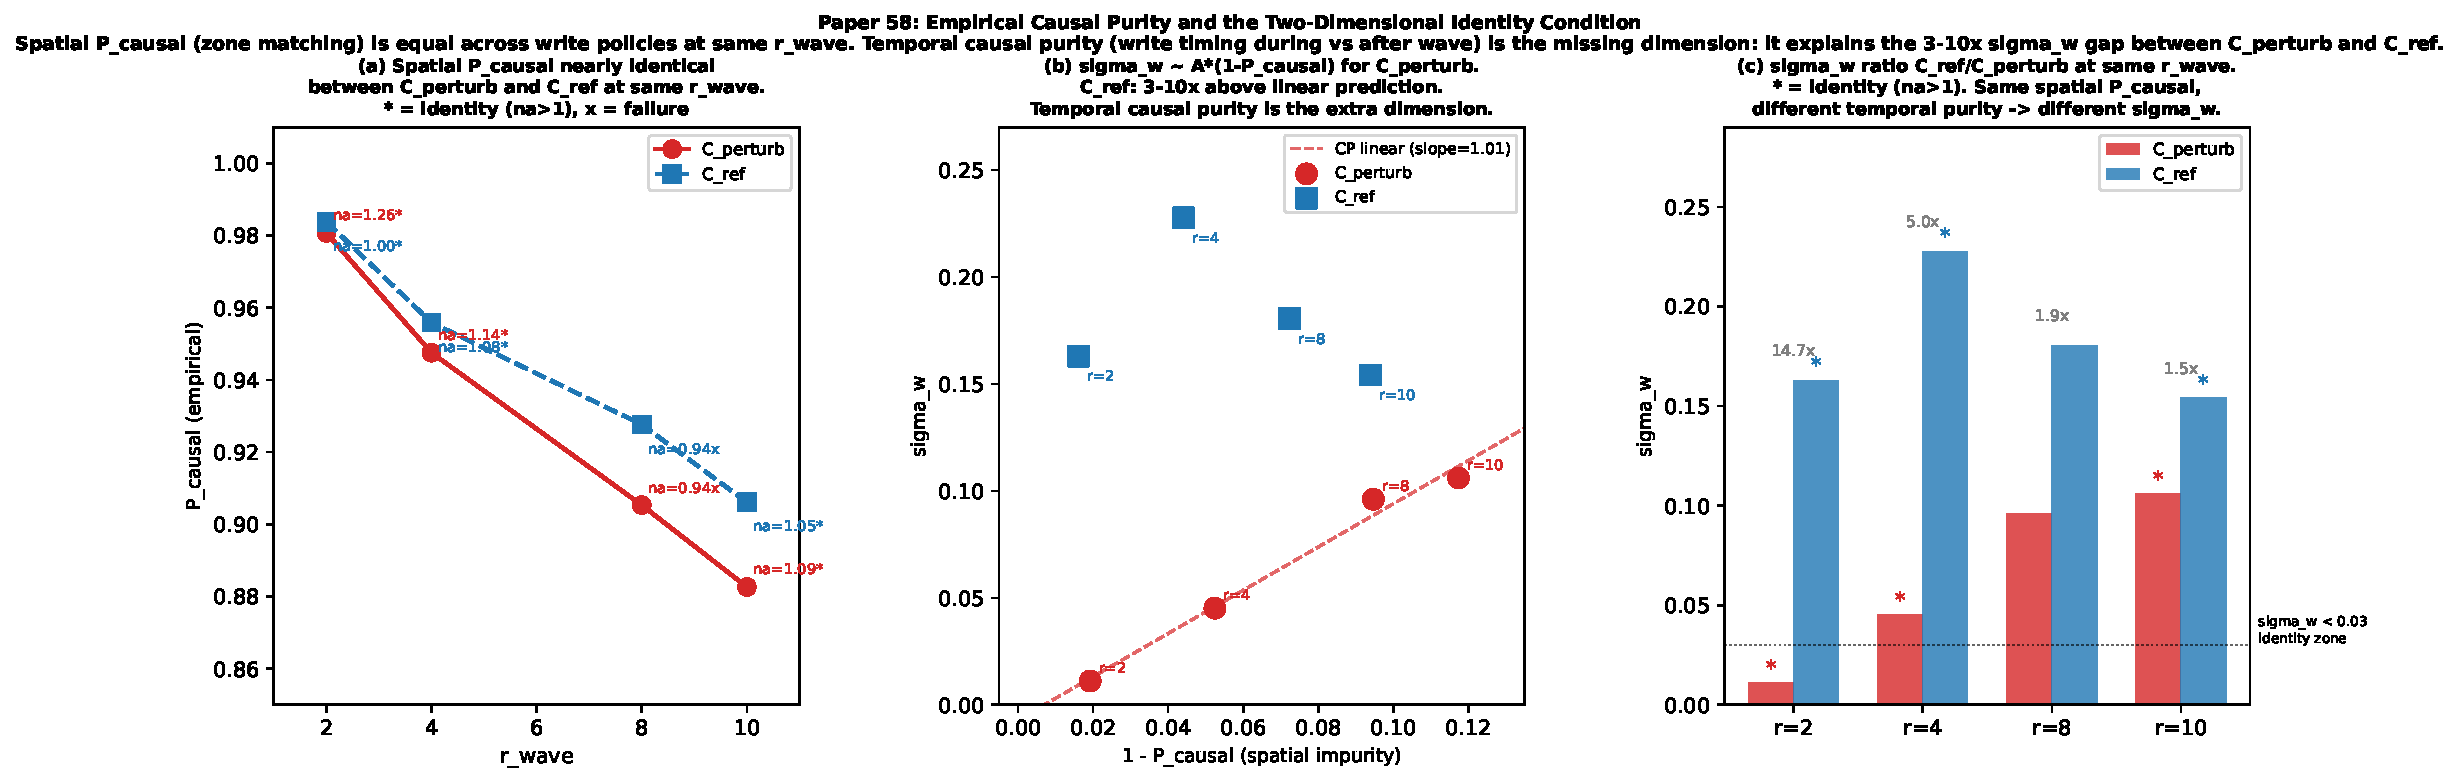
\includegraphics[width=\linewidth]{paper58_figure1.pdf}
  \caption{(a) Empirical $\Psp$ vs.\ $r_\mathrm{wave}$: C\_perturb and C\_ref are nearly
    indistinguishable, both decreasing with $r_\mathrm{wave}$. Identity outcome (na$>1$: *,
    failure: x) is not predicted by $\Psp$ alone.
    (b) $\sigma_w$ vs.\ $(1 - \Psp)$: linear model holds for C\_perturb (constant slope
    $A \approx 0.84$, dashed fit), breaks for C\_ref (ratios 1.6--10$\times$ above linear).
    (c) $\sigma_w$ side-by-side at same $r_\mathrm{wave}$: numbers show the C\_ref/C\_perturb
    ratio (3--10$\times$). Same spatial purity, different temporal purity.}
  \label{fig:main}
\end{figure}

\end{document}
